\documentclass[letterpaper,12pt]{article}

\usepackage[utf8]{inputenc}
\usepackage[T1]{fontenc}
\usepackage{lmodern}
\usepackage[french,english]{babel}
\usepackage[margin=1in]{geometry}
\usepackage{amsmath,amssymb,bm}
\usepackage{array,booktabs,longtable}
\usepackage[dvipsnames]{xcolor}
\usepackage{enumitem}
\usepackage{graphicx}
\usepackage[section]{placeins}
\usepackage{siunitx}
\usepackage[most]{tcolorbox}
% Section, table and page numbers of the thesis come from ../Document.aux, so they always
% match the final version. Build the thesis first (make), then this file.
\usepackage{xr-hyper}
\usepackage[hidelinks]{hyperref}
\externaldocument[T-]{../Document}

\graphicspath{{../images/}}
\setlength{\parskip}{0.5em}
\setlength{\parindent}{0pt}

% The thesis notation (defs.tex) and its acronyms, spelled out here.
% text abbrevs
\newcommand{\eg}{{\it e.g.}}
\newcommand{\ie}{{\it i.e.}}
\newcommand{\etc}{{\it etc.}}

\newcommand{\BEQ}{\begin{equation}}
\newcommand{\EEQ}{\end{equation}}
\newcommand{\BEAS}{\begin{eqnarray*}}
\newcommand{\EEAS}{\end{eqnarray*}}
% std math stuff
% Notation scheme (advisor, 2026-07-30): number sets in \mathbb, general sets in \mathcal,
% vectors lowercase \mathbf, matrices uppercase \mathbf, Greek vectors in \bm.
\newcommand{\ones}{\mathbf 1}
\newcommand{\zeros}{\mathbf 0}
\newcommand{\reals}{\mathbb{R}}
\newcommand{\integers}{\mathbb{Z}}
\newcommand{\eqbydef}{\mathrel{\stackrel{\Delta}{=}}}
\newcommand{\complex}{\mathbb{C}}
\newcommand{\symm}{\mathbb{S}}  % symmetric matrices
\newcommand{\mvec}[1]{\mathbf{#1}}   % vectors (latin): \mvec{x}
\newcommand{\mmat}[1]{\mathbf{#1}}   % matrices: \mmat{A}
\newcommand{\gvec}[1]{\bm{#1}}       % vectors (greek): \gvec{\theta}
\newcommand{\cone}[1]{\mathcal{#1}}  % cones and general sets: \cone{K}
\newcommand{\sign}{{\mbox{\bf sign}}}
\newcommand{\sinc}{{\mbox{\bf sinc}}} 

\newcommand{\Div}{\nabla \!\cdot\!}

% lin alg stuff
\newcommand{\Span}{\mbox{\textrm{span}}}
\newcommand{\Range}{\mbox{\textrm{range}}}
\newcommand{\nullspace}{{\mathcal N}}
\newcommand{\range}{{\mathcal R}}
\newcommand{\Nullspace}{\mbox{\textrm{nullspace}}}
\newcommand{\Rank}{\mathop{\bf Rank}}
\newcommand{\Tr}{\mathop{\bf Tr}}
\newcommand{\diag}{\mathop{\mathrm{diag}}}
\newcommand{\lambdamax}{{\lambda_{\rm max}}}
\newcommand{\lambdamin}{\lambda_{\rm min}}
%XXX dumb question: do we not use \diag(...) to form diagonal or
%block diagonal matrices?

% probability stuff
\newcommand{\Expect}{\mathop{\bf E{}}}
\newcommand{\expect}[1]{\mathop{\bf E{}}[#1]}
\newcommand{\Prob}{\mathop{\bf Prob}}
\newcommand{\erf}{\mathop{\bf erf}}

% convexity & optimization stuff
\newcommand{\Co}{{\mathop {\bf Co}}}
\newcommand{\co}{{\mathop {\bf Co}}}
% \newcommand{\Var}{\mathop{\bf var{}}}
\newcommand{\dist}{\mathop{\bf dist{}}}
\newcommand{\Ltwo}{{\bf L}_2}
%\newcommand{\QED}{~~\rule[-1pt]{8pt}{8pt}}\def\qed{\QED}
\newcommand{\approxleq}{\mathrel{\smash{\makebox[0pt][l]{\raisebox{-3.4pt}{\small$\sim$}}}{\raisebox{1.1pt}{$<$}}}}
\newcommand{\argmin}{\mathop{\rm argmin}}
\newcommand{\epi}{\mathop{\bf epi}}
\newcommand{\hypo}{\mathop{\bf hypo}}
\newcommand{\var}{\mathop{\bf var}}
\newcommand{\avg}{\mathop{\bf avg}}

\newcommand{\vol}{\mathop{\bf vol}}
\newcommand{\Vol}{\mathop{\bf vol}}
\newcommand{\Card}{\mathop{\bf card}}

\newcommand{\dom}{\mathop{\bf dom}}
\newcommand{\aff}{\mathop{\bf aff}}
\newcommand{\cl}{\mathop{\bf cl}}
\newcommand{\Angle}{\mathop{\bf angle}}
\newcommand{\intr}{\mathop{\bf int}}
\newcommand{\relint}{\mathop{\bf rel int}}
\newcommand{\bd}{\mathop{\bf bd}}
\newcommand{\vect}{\mathop{\mathrm{vec}}}
\newcommand{\dsp}{\displaystyle}
\newcommand{\foequal}{\simeq}
\newcommand{\VOL}{{\mbox{\bf vol}}}
\newcommand{\argmax}{\mathop{\rm argmax}}
\newcommand{\xopt}{x^{\rm opt}}

\newcommand{\prox}{\mathbf{prox}}

\newcommand{\SURE}{\textrm{SURE}}
\newcommand{\SURECR}{\textrm{SURE-CR}}

\usepackage{relsize} % Relsize package needed
\usepackage{bm} % Bold greek for parameter vectors (\gvec)

\newcommand{\hutchpp}{\text{Hutch\raisebox{0.35ex}{\relscale{0.75}++}}}

%% new commands from CVXPY paper
\newcommand\plotzero{{\color{gray}0}}
\newcommand\annotatedop[2]{\phantom{\ensuremath{#2}}\hspace{2ex}\ensuremath{#1}\hspace{2ex}{\color{gray}\ensuremath{#2}}}

\newcommand{\ac}[1]{#1}

% A thesis reference: \tref{label} gives "§4.2, p. 61" from the thesis.
\newcommand{\tsec}[1]{\S\ref{T-#1}}
\newcommand{\tpage}[1]{p.~\pageref{T-#1}}
\newcommand{\tref}[1]{\tsec{#1}, \tpage{#1}}

% A committee question, our response, and the new text of the thesis, quoted.
\newcommand{\question}[2]{\FloatBarrier\par\bigskip\textbf{Q#1.} \emph{#2}\par}
\newtcolorbox{thesisquote}[1]{breakable, enhanced, colback=NavyBlue!4, colframe=NavyBlue!60,
  boxrule=0.4pt, arc=1pt, left=6pt, right=6pt, top=4pt, bottom=4pt, fontupper=\small,
  title={\small Changes in the thesis, #1}, coltitle=black, colbacktitle=NavyBlue!12}

\begin{document}

\begin{center}
{\Large\bfseries Response to the committee}\\[0.5em]
\emph{A Lightweight Canonicalization Engine in C for Disciplined Convex Programming}\\[0.3em]
William Zijie Zhang (2362162), Master's thesis, Electrical Engineering, Polytechnique
Montréal\\
Supervisor: Prof.~Antoine Lesage-Landry\\[0.3em]
\today
\end{center}

\noindent To Prof.~Sébastien Le Digabel (chair), Prof.~Antoine Legrain (second member) and
Prof.~Antoine Lesage-Landry (supervisor).

\begin{otherlanguage}{french}
\section*{Message au jury}

Bonjour chers membres du jury,

Je voulais tout d'abord vous remercier pour vos commentaires sur mon mémoire. Comme vous m'avez
demandé de clarifier et d'approfondir plusieurs points des résultats, j'ai pris le temps de les
rendre plus complets, et j'ai aussi découvert quelques erreurs dans les affirmations que j'avais
faites sur les contributions.

Premièrement, il y a maintenant quatre problèmes qui sont plus lents. J'explique la cause de
chacun au chapitre~4 (\S\ref{T-sec:bench-oneshot}), avec la part de chaque phase du temps, et
je donne le détail à la section~\ref{sec:supplement}. Trois des quatre problèmes peuvent devenir
plus rapides. Deux d'entre eux le deviennent avec des changements dans le «~frontend~» (par
frontend, je fais référence à la manipulation des arbres d'expression avant le calcul des
dérivées). Par exemple, pouvoir détecter que \texttt{D @ ones} (où \texttt{D} est une matrice
quelconque) équivaut à \texttt{D.sum(axis=1)}, la somme sur les colonnes, est un grand avantage.
Le troisième, ConvexPlasticity, le devient avec un test de densité. Ces changements ne règlent
pas tout : une partie du ralentissement vient de \texttt{SparseDiffEngine} lui-même (voir Q5).

Deuxièmement, j'ai refait toutes les mesures sur un ordinateur plus récent (MacBook M2 de 2022,
avec Apple \texttt{Accelerate}), plutôt que sur l'ordinateur Intel de 2018 de la version
soumise, pour que les résultats soient reproductibles sur du matériel actuel, comme celui de la
plupart des utilisateurs de \texttt{CVXPY}. Pour la première canonicalisation, les ratios et les
temps sont semblables. Pour les re-résolutions paramétriques, en revanche, \texttt{diffengine}
n'est plus rapide que sur trois des sept problèmes, contre cinq dans la version soumise. Sur
les quatre autres, la passe numérique ne prend que $4$ à $24\,\%$ d'une re-résolution ; le
reste est du post-traitement, après \texttt{SparseDiffEngine}. J'ai donc modifié les
affirmations de ma conclusion et de la discussion des résultats pour dire seulement qu'il y a
des bénéfices, mais que la séparation ne remplace pas encore le tenseur pour les re-résolutions.
En refaisant ces mesures avec les versions des logiciels de la version soumise, j'ai vérifié que
ce changement ne vient ni de l'ordinateur ni de \texttt{SparseDiffEngine}, mais de l'interface
entre \texttt{CVXPY} et \texttt{SparseDiffEngine}, en particulier d'une modification
postérieure à la version 1.9.2. Comme les autres backends sont mesurés avec la version 1.9.2,
les re-résolutions de \texttt{diffengine} sont maintenant mesurées sans cette modification
aussi. Réduire ce post-traitement est maintenant le premier des travaux futurs.

Troisièmement, le problème UnconstrainedQP n'était pas réellement 100 fois plus rapide. C'était
dû à un changement de frontend que j'avais appliqué sur la branche du backend
\texttt{diffengine}, mais pas sur celles des autres. En l'appliquant à tous, cet avantage
disparaît. Ceci a été rectifié : aucun backend n'utilise maintenant ce changement.

À part ces trois points, qui sont les changements majeurs, j'ai aussi fait les études
d'ablation et exécuté plus d'instances de benchmark, avec des mesures de signification
statistique, ce qui répond à tous vos commentaires.

J'ai rédigé des ébauches de réponses à vos questions, que Claude, l'outil d'IA déclaré dans le
mémoire, a ensuite peaufinées ; les chiffres viennent directement des scripts de mesure.
\end{otherlanguage}

\section{Summary of corrections}

I have made all the modifications required by the committee and by Prof.~Antoine Legrain's
examiner report, as well as the minor corrections that Prof.~Sébastien Le Digabel annotated and
those listed in the appendix of Prof.~Legrain's report. The minor corrections are not listed
here.
All changes since the version sent to the committee are marked in \texttt{Document-diff.pdf},
with added text in blue and deleted text in red. Section, table and page numbers below refer to
the final version.

Table~\ref{tab:required} lists the required modifications. ``J'' refers to the committee's
requirements after the defence, and (i)--(vii) to the items of the synthesis of the examiner
report. The defence questions are answered in Section~\ref{sec:replies}; the other items are
in the thesis sections listed.

{\small
\begin{longtable}{>{\raggedright}p{0.17\textwidth} >{\raggedright}p{0.50\textwidth}
  >{\raggedright\arraybackslash}p{0.25\textwidth}}
\caption{Required modifications and where they are made.}\label{tab:required}\\
\toprule
Request & Change & Where \\
\midrule
\endfirsthead
\toprule
Request & Change & Where \\
\midrule
\endhead
\bottomrule
\endfoot
J1a: statistical significance
  & $30$ runs per comparison; Mann--Whitney~\cite{mann1947} per problem,
    Holm-adjusted~\cite{holm1979}; Wilcoxon~\cite{wilcoxon1945} and a bootstrap interval over
    the suite.
  & Ch.~4 introduction, \tpage{sec:Theme2}; \tsec{sec:bench-oneshot} \\
J1b, (ii): ablation
  & Dense blocks turned off on all $25$ problems, in time and memory; the split ablated on the
    re-solves (Q2).
  & \tref{sec:bench-ablation}; Tables~\ref{tab:sup-nodense} and~\ref{tab:sup-memory} \\
J1c: more instances
  & New parameter values for each run, and every problem scaled in size and density.
  & Ch.~4 introduction; \tsec{sec:bench-sensitivity} \\
J1d: sensitivity to size and sparsity
  & All $25$ problems at five sizes and eight at seven densities, with and without the dense
    blocks.
  & \tref{sec:bench-sensitivity}; Figure~\ref{fig:sup-density} \\
J1e, (iii): non-DPP problems
  & Re-solves of two families in DPP, non-DPP and parameter-free variants, and of
    ConvexPlasticity (Q3).
  & \tref{sec:bench-nondpp} \\
J2, (i): related literature and DNLP
  & Matrix-free modelling, \texttt{CVXcanon}, \texttt{CVXGEN}, \texttt{Convex.jl}~0.16,
    \texttt{Pyomo}, block-sparse antecedents and sparse factorization; who leads
    \texttt{SparseDiffEngine} and what is specific to this work (Q6).
  & \S\ref{T-sec:computing-derivatives}, \tsec{sec:contributions},
    \tsec{sec:theme1-atom-classes} \\
J3: declaration of AI use
  & New front-matter page.
  & Front matter \\
(iv): repeated measurements
  & $30$ runs, each in a fresh process; tables give mean $\pm$ standard deviation.
  & Ch.~4 introduction; Table~\ref{T-tab:oneshot-compile} \\
(v): dimensions of the instances
  & Dimensions, nonzeros, density, parameter size and DPP status of every problem.
  & Appendix~\ref{T-app:bench}, Tables~\ref{T-tab:instances-desc} and~\ref{T-tab:instances} \\
(vi): time by phase
  & The share of each phase on the four slower problems, with the cause of each.
  & \tref{sec:bench-oneshot}; Table~\ref{tab:sup-phases} \\
(vii): correctness check
  & The problem data are checked against the \texttt{CPP} backend to a relative tolerance of
    $10^{-9}$, at the first canonicalization and after a parameter update.
  & Ch.~4 introduction \\
\end{longtable}}

\section{Replies to the defence questions}\label{sec:replies}

\question{1}{Why materialize dense blocks rather than leave them as operators, as in the
matrix-free approach of Diamond and Boyd~\cite{diamond2016matrixfree}? When is each approach
preferable?}
Because the solvers that \texttt{CVXPY} calls need the matrices. Its default solvers are
\texttt{Clarabel}, an interior-point method, and \texttt{OSQP} and \texttt{SCS}, which are
first-order methods; commercial solvers such as \texttt{MOSEK} and \texttt{Gurobi} are
interior-point or simplex methods. All of them factorize a matrix built from $\mmat{A}$ and
$\mmat{P}$: an interior-point method factorizes a KKT system at every iteration, and
\texttt{OSQP} and \texttt{SCS}, in their default direct mode, factorize their KKT matrix once and
reuse the factorization across iterations. So every one of them needs $\mmat{A}$ and $\mmat{P}$ explicitly,
whatever its algorithm. Matrix-free modelling pays off for very large problems built from fast
transforms, solved by first-order methods that only need products with $\mmat{A}$ and
$\mmat{A}^\top$, such as the indirect mode of \texttt{SCS}. A permuted dense block lies between
the two: it is a materialized matrix, but it keeps the structure of the operator, namely its
row and column selectors and its dense block.

\begin{thesisquote}{\tref{sec:computing-derivatives}}
In convex optimization, Diamond and Boyd take the matrix-free view. Instead of forming
$\mmat{A}$, they represent the problem as a graph of linear operators, available only through
their forward and adjoint products, which suits first-order solvers. The solvers that
\texttt{CVXPY} calls by default instead factorize a matrix built from $\mmat{A}$ and $\mmat{P}$.
The matrix-free approach pays off on very large problems built from fast transforms, such as
convolutions and Fourier transforms, and it needs solvers that accept operators instead of
matrices. The permuted dense matrices of \S3.2 sit between the two: they form the matrix that
the solver factorizes, but keep the structure of the operator, its row and column selectors and
its dense block.
\end{thesisquote}

\question{2}{If the permuted dense representations are disabled, what fraction of the speedup
remains?}
Most of it. Without the dense blocks, \texttt{diffengine} is $2.15\times$ faster than the best
\texttt{CVXPY} backend in geometric mean, against $2.29\times$ with them, and the difference is
not significant over the suite (Wilcoxon, $p = 0.07$). Per problem, however, the effect is large
in both directions (Table~\ref{T-tab:oneshot-compile} of the thesis; Tables~\ref{tab:sup-nodense} and~\ref{tab:sup-memory}):
the dense blocks help by
$1.8$ to $3\times$ on eight problems with dense data, and hurt by $1.4$ to $46\times$ on the
three that build a dense block from sparse data (CVaR, ConvexPlasticity, UnconstrainedQP).
Without them, \texttt{diffengine} also uses $0.83$ times the peak memory in geometric mean.

The dense blocks are the only part of the engine that can be turned off on a first
canonicalization; the implementation in C, one Jacobian per node and the global layout are built
into every atom, so we do not attribute the remaining $2.15\times$ to any one of them. The split
between the symbolic and numeric passes matters only on re-solves, where removing it makes a
re-solve $2.9\times$ slower, significantly on all seven problems
(Table~\ref{tab:res-ablation}). \emph{We conclude that most of the first-canonicalization
speedup comes from the engine as a whole rather than from the dense blocks, which should only be
built from data that is dense in fact, and that the re-solve speed comes from the split.}

\begin{table}[htbp]
\centering
\caption{The ablations in summary: geometric mean of the ratio of each variant to its
reference, its bootstrap $95\,\%$ confidence interval, the Wilcoxon $p$-value over the problems,
and the number of problems with a significant difference (Mann--Whitney, Holm-adjusted).}
\label{tab:res-ablation}
{\small
\begin{tabular}{l l r l l l}
\toprule
Variant & Reference & Ratio & 95\,\% CI & $p$ & Significant \\
\midrule
\multicolumn{6}{l}{\textit{First canonicalization, $25$ problems}} \\
no dense blocks        & \texttt{diffengine}  & 1.06 & 0.71--1.45 & 0.067 & 24/$25$ \\
no dense blocks        & best \texttt{CVXPY}  & 0.46 & 0.36--0.61 & $3.2 \times 10^{-5}$ & 25/$25$ \\
\addlinespace
\multicolumn{6}{l}{\textit{Re-solve, $7$ \ac{DPP} problems}} \\
no dense blocks        & \texttt{diffengine}  & 1.01 & 0.98--1.05 & 0.938 & 6/$7$ \\
no split               & \texttt{diffengine}  & 2.86 & 1.73--4.91 & 0.016 & 7/$7$ \\
neither                & \texttt{diffengine}  & 3.68 & 2.19--6.20 & 0.016 & 7/$7$ \\
\bottomrule
\end{tabular}}
\end{table}


\question{3}{How does re-solving behave on a non-DPP parametric problem?}
On the two families written with a product of two parameters, which \ac{DPP} forbids,
\texttt{CVXPY} has to canonicalize the problem again at every solve, while \texttt{diffengine}
keeps its symbolic pass and reruns only the numeric pass. It re-solves as fast as on the
\ac{DPP} variant, $13$ to $14\times$ faster than \texttt{CVXPY} on \texttt{lasso} and
\texttt{factor\_cov}, significantly on both (Table~\ref{tab:res-nondpp}). ConvexPlasticity,
the suite's only natural non-DPP parametric problem, is the exception: it re-solves in $207$~ms
against $42$~ms for \texttt{CVXPY}, because $88\,\%$ of the re-solve assembles a dense $3000
\times 3000$ block of $\mmat{P}$ built from a diagonal. Without the dense blocks, it re-solves
in $2.0$~ms, $21\times$ faster than \texttt{CVXPY}. The thesis no longer claims that the split
replaces the tensor (Q4).

\begin{table}[htbp]
\centering
\caption{Re-solve time in milliseconds, mean over $30$ runs; every standard deviation is
below $1\,\%$ of the mean. \texttt{factor\_cov} is FactorCovarianceModel with $n$ assets. The
non-DPP variant writes $\lambda$, or the risk aversion $\gamma$, as the product of two
parameters, and the parameter-free variant makes it a constant. \texttt{CVXPY} applies the
tensor on the DPP variant and canonicalizes again on the others; the cached column of
\texttt{diffengine} runs the numeric pass only, and the rebuild column the symbolic pass as
well. The ratio is the median of \texttt{diffengine}, cached when it can, over that of
\texttt{CVXPY}, $^{*}$ when significant. The thesis states these results in
\tsec{sec:bench-nondpp} without the table.}\label{tab:res-nondpp}
{\small
\begin{tabular}{l l r rr l}
\toprule
& & & \multicolumn{2}{c}{\texttt{diffengine}} & \\
\cmidrule(lr){4-5}
Family & Variant & \texttt{CVXPY} & cached & rebuild & Ratio \\
\midrule
\texttt{lasso}, $n = 1000$         & \ac{DPP}        & 6.4 & 23.3 & 32.7 & 3.64$^{*}$ \\
                                   & non-\ac{DPP}    & 315 & 23.3 & 32.8 & 0.07$^{*}$ \\
                                   & parameter-free  & 338 & --- & 49.0 & 0.14$^{*}$ \\
\addlinespace
\texttt{factor\_cov}, $n = 5000$   & \ac{DPP}        & 1.2 & 3.6 & 6.9 & 2.86$^{*}$ \\
                                   & non-\ac{DPP}    & 45.8 & 3.6 & 7.0 & 0.08$^{*}$ \\
                                   & parameter-free  & 47.1 & --- & 11.0 & 0.23$^{*}$ \\
\bottomrule
\end{tabular}}
\end{table}

\begin{thesisquote}{\tref{sec:bench-nondpp}}
On the non-\ac{DPP} variants, \texttt{CVXPY} canonicalizes again at every solve, while
\texttt{diffengine} reruns only its numeric pass and re-solves $13$ to $14$ times faster.
ConvexPlasticity, the only parametric problem of the suite that is not \ac{DPP}, is the
exception [\ldots]. Without the dense blocks, it re-solves in $2.0$ milliseconds, $21$ times
faster than \texttt{CVXPY}.
\end{thesisquote}
\begin{thesisquote}{\tref{sec:bench-summary}}
Caching canonicalization does not necessarily require the \ac{DPP} ruleset. [\ldots] the
symbolic and numeric split re-solves within a factor of four of the cached tensor on every
\ac{DPP} problem. [\ldots] it re-solves problems that are not \ac{DPP}, on which
\texttt{CVXPY} has to canonicalize again, $13$ to $14$ times faster.
\end{thesisquote}

\question{4}{Why not re-evaluate only the subtrees that depend on the updated parameters?}
The engine now does this: after a parameter update, the numeric pass re-evaluates only the
subtrees that contain a parameter, and keeps the cached values of the others. All re-solve
times in the thesis use it.

On the seven \ac{DPP} problems (Table~\ref{tab:res-param}), \texttt{diffengine} has the fastest
first canonicalization on all seven, $2.5$ to $6.6\times$ faster than the fastest tensor build.
The cached tensor re-solves faster on four of them, by $1.10$ to $3.60\times$, and recovers its
slower first canonicalization only after $18$ to $124$ re-solves. On those four, the numeric
pass takes only $4$ to $24\,\%$ of a re-solve; the rest is post-processing after the engine,
the conversion to the solver's format. \emph{We conclude that the split does not replace the
tensor on \ac{DPP} problems that are re-solved many times, but comes within a factor of four of
it without the \ac{DPP} rules.} Making the post-processing cheaper is now the first item of
future work.

\begin{table}[htbp]
\centering
\caption{Table~\ref{T-tab:param-tensor} of the thesis (\tpage{tab:param-tensor}): first
canonicalization in seconds and re-solve in milliseconds, mean over $30$ runs. A dash is a tensor
that exceeded the memory or time limit. The ratio is the median re-solve of
\texttt{diffengine} over that of the fastest tensor, $^{*}$ when significant.}
\label{tab:res-param}
{\footnotesize
\setlength{\tabcolsep}{4pt}
\begin{tabular}{l rrrr rr l}
\toprule
& \multicolumn{4}{c}{first canonicalization (s)} & \multicolumn{2}{c}{re-solve (ms)} & \\
\cmidrule(lr){2-5}\cmidrule(lr){6-7}
Benchmark & \texttt{CPP} & \texttt{SCIPY} & \texttt{COO} & \texttt{diffengine}
& tensor & \texttt{diffengine} & Ratio \\
\midrule
ParamSmallMatrixStuffing    & 2.02 & 7.30 & 0.083 & \textbf{0.033} & 1.8 & \textbf{0.4} & 0.24$^{*}$ \\
ParamConeMatrixStuffing     & 0.74 & 1.85 & 0.055 & \textbf{0.022} & 1.0 & \textbf{0.3} & 0.27$^{*}$ \\
SimpleFullyParametrizedLP   & --- & --- & 0.57 & \textbf{0.12} & 47 & \textbf{35} & 0.73$^{*}$ \\
SimpleScalarParametrizedLP  & 1.33 & 1.17 & 1.19 & \textbf{0.23} & \textbf{63} & 70 & 1.10$^{*}$ \\
ParametrizedQP              & --- & --- & 2.63 & \textbf{0.76} & \textbf{299} & 349 & 1.16$^{*}$ \\
SVMWithL1Regularization     & 2.80 & 2.57 & 2.83 & \textbf{0.39} & \textbf{38} & 125 & 3.26$^{*}$ \\
FactorCovarianceModel       & 1.20 & 1.14 & 1.19 & \textbf{0.18} & \textbf{21} & 74 & 3.60$^{*}$ \\
\bottomrule
\end{tabular}}
\end{table}

\begin{thesisquote}{\tref{sec:theme1-problem-interface}}
The numeric pass therefore skips an affine tree after the first evaluation, until the next
parameter update. After an update, it re-evaluates only the subtrees that contain a parameter,
and keeps the cached values of the others.
\end{thesisquote}

\question{5}{When does the global layout become a handicap relative to \texttt{CVXPY}'s local
layout, in particular for memory?}
When the problem has many variables and many nodes. In the global layout, each node keeps,
besides its Jacobian, integer work arrays of length $n$, the total number of variables, whatever
variables its own subtree contains. Their memory is therefore $O(\text{nodes} \times n)$
integers. In \texttt{CVXPY}'s local layout, each node stores blocks only for the variables it
depends on, so the same overhead is proportional to the sum, over the nodes, of the number of
variables each one depends on. The two coincide when every node depends on every variable, and
the local layout wins when most nodes depend on a few variables out of many.

OptimalAdvertising shows it. Each of its $250$ minimum terms depends on one row of a
$250 \times 1000$ variable, but has a Jacobian over all $250\,000$ variables. Without the dense
blocks, its peak memory is $945$~MB, against $173$ to $197$~MB for the \texttt{CVXPY} backends.
With them it reaches $6.1$~GB, because each dense block of the aggregate constraints
$\mmat{D}^\top \ones \le \mvec{t}$ and $\mmat{D} \ones \ge \mvec{c}$ also keeps one integer per
variable of the problem: the same cost, paid per block rather than per node. Rewriting these
products with a vector of ones as sums avoids the dense blocks: OptimalAdvertising then
canonicalizes in $0.33$~s instead of $0.91$~s, faster than the $0.53$~s of \texttt{CVXPY}, with
$1.4$~GB instead of $6.1$~GB. Storing the per-block maps sparsely would fix the general case.


\question{6}{What part of \texttt{SparseDiffEngine} pre-existed the thesis or was developed for
DNLP, and what part is specific to this work?}
Daniel Cederberg leads \texttt{SparseDiffEngine}. He started it as the differentiation engine
of the \texttt{DNLP} extension of \texttt{CVXPY}~\cite{cederberg2025disciplined}, which
differentiates nonlinear atoms at every iterate of the solver, and I co-developed it with him.
The version sent to the committee should have said so clearly; it
now does. This thesis uses the engine for a different
purpose, canonicalization: it evaluates the affine atoms and the quadratic form at the origin to
obtain the problem data. What is specific to the thesis is the interface to \texttt{CVXPY},
namely the \texttt{diffengine} backend and its re-solve path for parametric problems, and the
benchmarks of Chapter~4.

\begin{thesisquote}{\tref{sec:contributions}}
Daniel Cederberg is the lead developer of \texttt{SparseDiffEngine}. It was first built as the differentiation engine of the
\texttt{DNLP} extension of \texttt{CVXPY}, where it differentiates nonlinear atoms such as
\texttt{exp}, \texttt{log} and \texttt{entr} at every iterate of the solver. This thesis builds
on the observation that canonicalization is a special case of the same computation: once a
problem is canonicalized, only affine atoms and quadratic forms remain, and their derivatives
are the problem data.
\end{thesisquote}
\begin{thesisquote}{\tref{sec:theme1-atom-classes}}
What is specific to this thesis is the interface to \texttt{CVXPY} of \S3.3, namely the
\texttt{diffengine} backend and its re-solve path for parametric problems, and the benchmarks of
Chapter~4.
\end{thesisquote}

\question{7}{What is the strategy for \ac{BLAS} and binary distribution of
\texttt{sparsediffpy}?}
\texttt{cvxcore} is a C++ extension that lives inside the \texttt{CVXPY} repository, so
\texttt{CVXPY} has to compile and ship it. \texttt{sparsediffpy} is a separate package that
\texttt{CVXPY} only depends on. Its compiled wheels for Linux, macOS and Windows are published
on \texttt{PyPI}; they link Apple's \texttt{Accelerate} on macOS and bundle \texttt{OpenBLAS}
elsewhere, so users install nothing beyond the package.


\section{New and revised tables}

The thesis adds the two tables of Appendix~\ref{T-app:bench} and redoes two existing tables
with the new measurements. The other results are stated in the text, with the full measurements
in Section~\ref{sec:supplement}.

{\small
\begin{longtable}{>{\raggedright}p{0.17\textwidth} >{\raggedright}p{0.50\textwidth}
  >{\raggedright\arraybackslash}p{0.25\textwidth}}
\caption{Tables added to the thesis, or revised.}\label{tab:new-items}\\
\toprule
Item & Content & Request \\
\midrule
\endfirsthead
\toprule
Item & Content & Request \\
\midrule
\endhead
\bottomrule
\endfoot
Table~\ref{T-tab:oneshot-compile}
  & Revised: first canonicalization of the $25$ problems, now mean $\pm$ standard deviation over
    $30$ runs with significance, and the ratio without the dense blocks,
    \tpage{tab:oneshot-compile}
  & J1a, J1b, (ii), (iv) \\
Table~\ref{T-tab:param-tensor}
  & Revised: first canonicalization and re-solve of the \ac{DPP} problems, with standard
    deviations and significance,
    \tpage{tab:param-tensor}
  & J1a, (iv), Q4 \\
Table~\ref{T-tab:instances-desc}
  & The $25$ benchmark problems, \tpage{tab:instances-desc}
  & (v) \\
Table~\ref{T-tab:instances}
  & Dimensions of the benchmark problems, \tpage{tab:instances}
  & (v) \\
\end{longtable}}

\section{Supplementary results}\label{sec:supplement}

The thesis states the results below in a few sentences each; the full measurements are given
here for the committee. All are measured as in Chapter~\ref{T-sec:Theme2}, in $30$ runs.

\subsection*{Dense blocks: per problem (J1b, (ii), Q2)}

{\small
\begin{longtable}{l rr l rr}
\caption{First canonicalization of \texttt{diffengine} with and without the dense blocks, in
milliseconds. The ratio is the median time without the dense blocks over that with them,
$^{*}$ when significant (Mann--Whitney, Holm-adjusted $p < 0.05$). The last two columns are the
ratio of \texttt{diffengine} to the best \texttt{CVXPY} backend, as in
Table~\ref{T-tab:oneshot-compile} of the thesis.}\label{tab:sup-nodense}\\
\toprule
& & & & \multicolumn{2}{c}{to best \texttt{CVXPY}} \\
\cmidrule(lr){5-6}
Benchmark & \texttt{diffengine} & no dense blocks & Ratio & with & without \\
\midrule
\endfirsthead
\toprule
Benchmark & \texttt{diffengine} & no dense blocks & Ratio & with & without \\
\midrule
\endhead
\bottomrule
\endfoot
\multicolumn{6}{l}{\textit{Dense blocks help}} \\
SVMWithL1Regularization & 387 $\pm$ 1 & 745 $\pm$ 5 & 1.92$^{*}$ & 0.15 & 0.28 \\
FactorCovarianceModel & 177 $\pm$ 3 & 366 $\pm$ 6 & 2.06$^{*}$ & 0.15 & 0.32 \\
Yitzhaki & 145 $\pm$ 1 & 263 $\pm$ 1 & 1.82$^{*}$ & 0.15 & 0.28 \\
SimpleQP & 453 $\pm$ 1 & 914 $\pm$ 6 & 2.01$^{*}$ & 0.16 & 0.32 \\
HuberRegression & 495 $\pm$ 8 & 1\,015 $\pm$ 3 & 2.06$^{*}$ & 0.18 & 0.37 \\
LeastSquares & 435 $\pm$ 2 & 906 $\pm$ 2 & 2.08$^{*}$ & 0.18 & 0.38 \\
SimpleLP & 1\,121 $\pm$ 3 & 1\,485 $\pm$ 5 & 1.32$^{*}$ & 0.19 & 0.25 \\
ConeMatrixStuffing & 642 $\pm$ 4 & 1\,941 $\pm$ 7 & 3.03$^{*}$ & 0.30 & 0.90 \\
SmallMatrixStuffing & 502 $\pm$ 2 & 1\,369 $\pm$ 6 & 2.73$^{*}$ & 0.30 & 0.81 \\
ParamSmallMatrixStuffing & 32.7 $\pm$ 0.1 & 40.4 $\pm$ 0.3 & 1.23$^{*}$ & 0.52 & 0.64 \\
ParamConeMatrixStuffing & 22.4 $\pm$ 0.4 & 27.4 $\pm$ 0.7 & 1.22$^{*}$ & 0.52 & 0.64 \\
SDPSegfault1132 & 2\,147 $\pm$ 6 & 3\,466 $\pm$ 15 & 1.61$^{*}$ & 1.32 & 2.12 \\
\addlinespace
\multicolumn{6}{l}{\textit{Little effect}} \\
SimpleScalarParametrizedLP & 230 $\pm$ 1 & 225 $\pm$ 0.3 & 0.98$^{*}$ & 0.21 & 0.21 \\
SimpleFullyParametrizedLP & 115 $\pm$ 0.5 & 115 $\pm$ 0.4 & 1.00$^{*}$ & 0.22 & 0.22 \\
SlowPruning & 408 $\pm$ 1 & 417 $\pm$ 1 & 1.02$^{*}$ & 0.23 & 0.23 \\
ParametrizedQP & 755 $\pm$ 46 & 746 $\pm$ 34 & 1.00 & 0.25 & 0.25 \\
Cajas & 205 $\pm$ 1 & 209 $\pm$ 1 & 1.02$^{*}$ & 0.30 & 0.30 \\
TvInpainting & 257 $\pm$ 1 & 250 $\pm$ 1 & 0.97$^{*}$ & 0.32 & 0.31 \\
SemidefiniteProgramming & 405 $\pm$ 3 & 406 $\pm$ 1 & 1.00$^{*}$ & 0.64 & 0.64 \\
QuantumHilbertMatrix & 653 $\pm$ 3 & 671 $\pm$ 3 & 1.03$^{*}$ & 0.83 & 0.85 \\
Murray & 1\,181 $\pm$ 1 & 1\,179 $\pm$ 2 & 1.00$^{*}$ & 0.96 & 0.96 \\
OptimalAdvertising & 901 $\pm$ 4 & 834 $\pm$ 1 & 0.93$^{*}$ & 1.68 & 1.56 \\
\addlinespace
\multicolumn{6}{l}{\textit{Dense blocks hurt}} \\
CVaR & 3\,421 $\pm$ 9 & 2\,419 $\pm$ 36 & 0.71$^{*}$ & 0.53 & 0.37 \\
ConvexPlasticity & 507 $\pm$ 1 & 97.1 $\pm$ 3.2 & 0.19$^{*}$ & 7.31 & 1.39 \\
UnconstrainedQP & 22\,937 $\pm$ 21 & 500 $\pm$ 2 & 0.02$^{*}$ & 11.73 & 0.26 \\
\midrule
\textbf{Geometric mean} & & & \textbf{1.06} & \textbf{0.44} & \textbf{0.46} \\
\end{longtable}}

{\small
\begin{longtable}{l rrrrr}
\caption{Growth of the peak resident memory during the first canonicalization, in megabytes.
The last column is \texttt{diffengine} without the dense blocks.}\label{tab:sup-memory}\\
\toprule
Benchmark & \texttt{CPP} & \texttt{SCIPY} & \texttt{COO} & \texttt{diffengine} &
no dense blocks \\
\midrule
\endfirsthead
\toprule
Benchmark & \texttt{CPP} & \texttt{SCIPY} & \texttt{COO} & \texttt{diffengine} &
no dense blocks \\
\midrule
\endhead
\bottomrule
\endfoot
SVMWithL1Regularization & 1\,976 & 2\,041 & 2\,904 & 2\,034 & 2\,417 \\
FactorCovarianceModel & 1\,129 & 1\,047 & 1\,334 & 760 & 999 \\
Yitzhaki & 449 & 437 & 504 & 476 & 572 \\
SimpleQP & 2\,194 & 2\,355 & 3\,236 & 1\,655 & 2\,204 \\
HuberRegression & 2\,223 & 2\,246 & 3\,121 & 1\,413 & 1\,866 \\
LeastSquares & 2\,142 & 2\,327 & 3\,021 & 1\,459 & 1\,893 \\
SimpleLP & 5\,353 & 4\,961 & 5\,027 & 4\,792 & 5\,057 \\
SimpleScalarParametrizedLP & 1\,088 & 1\,024 & 1\,068 & 1\,009 & 1\,009 \\
SimpleFullyParametrizedLP & 517 & 494 & 526 & 492 & 492 \\
SlowPruning & 1\,352 & 1\,425 & 1\,828 & 1\,797 & 1\,120 \\
ParametrizedQP & 2\,035 & 2\,174 & 2\,998 & 1\,775 & 1\,775 \\
Cajas & 1\,193 & 298 & 320 & 341 & 342 \\
ConeMatrixStuffing & 2\,010 & 964 & 3\,730 & 478 & 1\,623 \\
SmallMatrixStuffing & 1\,189 & 634 & 2\,405 & 322 & 1\,117 \\
TvInpainting & 705 & 858 & 994 & 1\,048 & 1\,048 \\
ParamSmallMatrixStuffing & 17.4 & 12.4 & 21.9 & 10.6 & 10.5 \\
ParamConeMatrixStuffing & 9.8 & 8.2 & 12.2 & 5.9 & 5.8 \\
CVaR & 4\,022 & 2\,804 & 3\,587 & 10\,654 & 2\,115 \\
SemidefiniteProgramming & 1\,317 & 350 & 640 & 1\,138 & 1\,138 \\
QuantumHilbertMatrix & 222 & 218 & 288 & 1\,194 & 1\,194 \\
Murray & 2\,849 & 220 & 305 & 306 & 307 \\
SDPSegfault1132 & 7\,536 & 3\,460 & 15\,628 & 10\,413 & 12\,885 \\
OptimalAdvertising & 173 & 182 & 197 & 6\,066 & 945 \\
ConvexPlasticity & 82.5 & 82.5 & 82.3 & 1\,329 & 25.5 \\
UnconstrainedQP & 1\,427 & 1\,058 & 2\,105 & 1\,754 & 644 \\
\end{longtable}}

\subsection*{Density sweep (J1d)}

The data matrix of eight problems is multiplied entrywise by a random $0/1$ mask with a fraction
$\rho$ of ones, and stays a dense array, as it would be in a user's code.
Figure~\ref{fig:sup-density} shows four of them; FactorCovarianceModel, SimpleQP, Yitzhaki and
\texttt{lasso} follow the pattern of LeastSquares.

\begin{figure}[htbp]
\centering
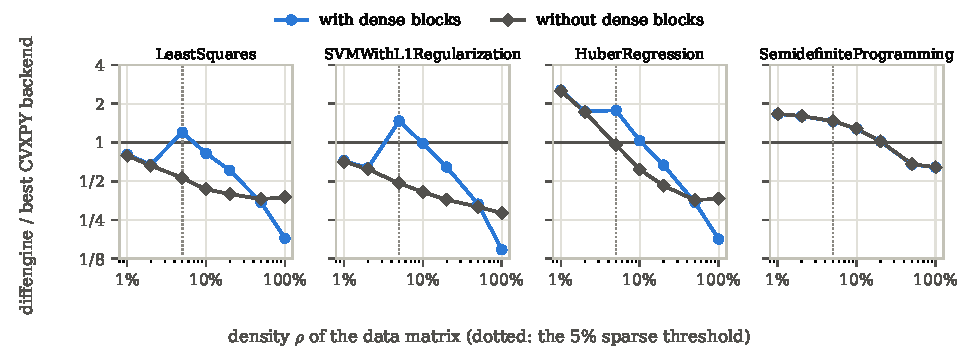
\includegraphics[width=\textwidth]{density_thesis}
\caption{Ratio of the median canonicalization time of \texttt{diffengine} to that of the best
\texttt{CVXPY} backend as the density $\rho$ of the data matrix falls, with and without the dense
blocks. The dotted line is the $5\,\%$ density below which \texttt{diffengine} stores a constant
factor in the sparse format. Every difference is significant (Mann--Whitney, Holm-adjusted over
the problems of each density).}\label{fig:sup-density}
\end{figure}

\subsection*{The four slower problems ((vi), Q5)}

On the four problems on which \texttt{diffengine} is slower, the cause lies in how their data
reaches the engine. Table~\ref{tab:sup-phases} gives the share of each phase of its first
canonicalization. Three of the four are addressed by changes to \texttt{CVXPY}, described
below, which the measurements of the thesis do not include; each fix is measured alone.

\begin{table}[htbp]
\centering
\caption{Phases of the first canonicalization of \texttt{diffengine} on the four slower
problems, in percent of its time, and the median share over the $25$ problems.}
\label{tab:sup-phases}
{\small
\setlength{\tabcolsep}{4pt}
\begin{tabular}{l r rrrrrr}
\toprule
Benchmark & Time (s) & Front end & Convert & Symbolic & Numeric & Assemble & Format \\
\midrule
UnconstrainedQP      & 22.94 & 0 & 0 & 2 & 98 & 0 & 0 \\
ConvexPlasticity     & 0.51 & 6 & 2 & 47 & 6 & 38 & 0 \\
OptimalAdvertising   & 0.90 & 4 & 1 & 89 & 4 & 1 & 1 \\
SDPSegfault1132      & 2.15 & 0 & 0 & 49 & 47 & 3 & 0 \\
\midrule
Median, all $25$     & ---  & 4 & 9 & 19 & 14 & 12 & 12 \\
\bottomrule
\end{tabular}}
\end{table}

\paragraph{UnconstrainedQP.} The problem minimizes
$\lVert \mmat{F}^{\mathsf{H}} \mmat{E}(\mvec{z}) \mmat{F} \mvec{x} - \mvec{y} \rVert_2$, with
$\mmat{E}(\mvec{z}) = \mmat{I}_{14} \otimes \diag(\mvec{z})$, over $\mvec{z} \in \complex^{18}$,
where $\mmat{F}$ is the $252 \times 252$ discrete Fourier transform matrix. Evaluated from the
left, the product $(\mmat{F}^{\mathsf{H}} \mmat{E}) \mmat{F}$ has a dense Jacobian of
$63\,504 \times 36$ entries, which the numeric pass fills one entry at a time. Evaluated from
$\mvec{x}$, as the reassociation of matrix products excluded from the thesis measurements does,
every intermediate is a vector, and the canonicalization takes $16$ milliseconds instead of
$22.9$ seconds, with a peak memory of $53$ megabytes instead of $1.75$ gigabytes.

\paragraph{OptimalAdvertising.} The problem maximizes
$\sum_{i=1}^{250} \min(r_i \mvec{p}_i^\top \mvec{d}_i, b_i)$ subject to $\mmat{D} \ge \zeros$,
$\mmat{D}^\top \ones \le \mvec{t}$ and $\mmat{D} \ones \ge \mvec{c}$, over
$\mmat{D} \in \reals^{250 \times 1000}$ with rows $\mvec{d}_i^\top$. Each minimum term depends
on one row of $\mmat{D}$, but its Jacobian spans all $250\,000$ variables, and the symbolic pass
visits every column of it, so its cost grows with the number of terms times the number of
variables. The two aggregate constraints are written as products with a vector of ones, which
become dense blocks. A change to \texttt{CVXPY} lowers them to sums, which reduces the
canonicalization from $0.91$ to $0.33$ seconds, below the $0.53$ seconds of the fastest
\texttt{CVXPY} backend, and the peak memory from $6.1$ to $1.4$ gigabytes.

\paragraph{SDPSegfault1132.} Three dense blocks of $49.5$ million entries cancel in a sum with
$1.01$ million nonzeros, and \texttt{diffengine} carries the cancelled entries through both
passes.

\paragraph{ConvexPlasticity.} The diagonal $h \mmat{I}$ of the quadratic objective is given as a
dense array and becomes a dense $3000 \times 3000$ block of $\mmat{P}$. A change to
\texttt{CVXPY} stores $\mmat{P}$ sparse below $5\,\%$ nonzeros, as is already done for a
constant factor of a matrix product, which reduces the canonicalization from $509$ to $203$
milliseconds and the peak memory from $1.33$ to $0.59$ gigabytes. The problem remains $2.9$
times slower than on the fastest \texttt{CVXPY} backend, and most of the remaining time is in
the symbolic pass.

\subsection*{Re-solve against a full canonicalization (Q4)}

{\footnotesize
\setlength{\tabcolsep}{4pt}
\begin{longtable}{l rr r}
\caption{Re-solve time in milliseconds on the seven \ac{DPP} problems: the cached tensor of
\texttt{CVXPY}, a full canonicalization on the \texttt{ignore\_dpp} path, both with the fastest
backend, and the cached re-solve of \texttt{diffengine}.}\label{tab:sup-warm}\\
\toprule
& \multicolumn{2}{c}{\texttt{CVXPY}} & \texttt{diffengine} \\
\cmidrule(lr){2-3}\cmidrule(lr){4-4}
Benchmark & tensor & recompile & cached \\
\midrule
\endfirsthead
\toprule
Benchmark & tensor & recompile & cached \\
\midrule
\endhead
\bottomrule
\endfoot
ParamSmallMatrixStuffing & 1.84 $\pm$ 0.01 & 57.6 $\pm$ 0.2 & 0.438 $\pm$ 0.007 \\
ParamConeMatrixStuffing & 0.958 $\pm$ 0.005 & 37.7 $\pm$ 0.2 & 0.265 $\pm$ 0.004 \\
SimpleFullyParametrizedLP & 46.7 $\pm$ 0.1 & 519 $\pm$ 1 & 34.6 $\pm$ 0.8 \\
SimpleScalarParametrizedLP & 62.8 $\pm$ 0.3 & 1\,078 $\pm$ 2 & 70.4 $\pm$ 5.9 \\
ParametrizedQP & 299 $\pm$ 8 & 2\,868 $\pm$ 14 & 349 $\pm$ 16 \\
SVMWithL1Regularization & 38.3 $\pm$ 0.1 & 2\,570 $\pm$ 3 & 125 $\pm$ 2 \\
FactorCovarianceModel & 20.5 $\pm$ 0.1 & 1\,138 $\pm$ 3 & 74.2 $\pm$ 0.8 \\
\end{longtable}}

\bibliographystyle{IEEEtran}
\bibliography{../Document}

\end{document}
